\documentclass[a4paper,12pt]{article} % тип документа

% Поля страниц
\usepackage[left=2.5cm,right=2.5cm,
    top=2cm,bottom=2cm,bindingoffset=0cm]{geometry}
    
%Пакет дял таблиц   
\usepackage{multirow} 
    
%Отступ после заголовка    
\usepackage{indentfirst}

% Математика
\usepackage{floatrow}
\floatsetup[table]{style=Plaintop}

% \usepackage{hyperref}
\usepackage[warn]{mathtext} %позволяет добавлять кириллицу в формулы

\usepackage{amsmath,amsfonts,amssymb,amsthm,mathtools} 
\usepackage{wasysym}
\usepackage[warn]{mathtext}
\usepackage{multicol}
\usepackage{graphicx}
\usepackage[shortcuts,cyremdash]{extdash}
\usepackage{wrapfig} % обтекание текстом
\usepackage{floatflt}
\usepackage{lipsum}
\usepackage{verbatim}
\usepackage{xcolor}
\usepackage{etoolbox}
\usepackage{subfiles}
\usepackage{enumitem}
\usepackage{amsthm}

% Рисунки
\usepackage{floatrow,graphicx,calc}
\usepackage{wrapfig}

%%% Работа с картинками
\usepackage{graphicx}  % Для вставки рисунков
\graphicspath{{images/}{images2/}}  % папки с картинками
\setlength\fboxsep{3pt} % Отступ рамки \fbox{} от рисунка
\setlength\fboxrule{1pt} % Толщина линий рамки \fbox{}
\usepackage{wrapfig} % Обтекание рисунков и таблиц текстом

\renewcommand{\arctan}{\mathop{\mathrm{arctg}}\nolimits}
\newcommand{\divisible}{\mathop{\raisebox{-2pt}{\vdots}}}
\newcommand{\grad}{\mathop{\mathrm{grad}}\nolimits}
\newcommand{\diver}{\mathop{\mathrm{div}}\nolimits}
\newcommand{\rot}{\mathop{\mathrm{rot}}\nolimits}
\newcommand{\veci}{{\vec\imath}}                % i-орт
\newcommand{\vecj}{{\vec\jmath}}                % j-орт
\newcommand{\veck}{{\vec{k}}}                   % k-орт
\renewcommand{\phi}{\varphi}                    % Красивая фи
\newcommand{\der}[2]{\frac{d #1}{d #2}} % derivative
\newcommand{\dpart}[2]{\frac{\partial #1}{\partial #2}} % first partial der
\newcommand{\ddpart}[2]{\frac{\partial^2 #1}{\partial #2^2}} % вторая частная производная
\newcommand{\e}{\mathop{\mathrm e}\nolimits}    % Экспонента
\newcommand{\E}{\mathcal{E}}                    % ЭДС
\renewcommand{\epsilon}{\varepsilon}            % Красивый эпсилон
\newcommand{\degr}{\ensuremath{^\circ}}         % Градус
\newcommand{\const}{\text{const}} % постоянная
\newcommand{\Int}{\int\limits}          % Большой интеграл (можно поменять \int на \varint)
\newcommand{\IInt}{\iint\limits}          % Большой интеграл (можно поменять \int на \varint)
\newcommand{\Oint}{\oint\limits}                % Большой интеграл
\newcommand{\lvec}[1]{\overrightarrow{#1}}            % beauty vector arrow
\newcommand{\quot}[1]{<<#1>>}                   % russian quotes
\newcommand{\iu}{\imath}
\newcommand{\system}[1]{\left\lbrace\begin{array}{c} #1 \end{array} \right.}
\newcommand{\orsys}[1]{\left[\begin{array}{c} #1 \end{array} \right.}

\newcommand{\cvec}[1]{\left[\begin{array}{c} #1 \end{array} \right]}
\newcommand{\matr}[2]{\left(\begin{array}{#1} #2 \end{array} \right)}
\newcommand{\matrtwo}[1]{\matr{c c}{#1}}
\newcommand{\matrthree}[1]{\matr{c c c}{#1}}
\newcommand{\detmat}[2]{\left|\begin{array}{#1} #2 \end{array} \right|}
\newcommand{\dettwo}[1]{\detmat{c c}{#1}}
\newcommand{\detthree}[1]{\detmat{c c c}{#1}}
\newcommand{\gath}[1]{\begin{gathered} 	#1	\end{gathered}}

\newcommand{\mean}[1]{\langle #1 \rangle}

\newcommand{\RomanNumeralCaps}[1] {\MakeUppercase{\romannumeral #1}}

% Создаёем новый разделитель
\DeclareFloatSeparators{mysep}{\hspace{1cm}}

% Ссылки?
\usepackage{hyperref}
\usepackage[rgb]{xcolor}
\hypersetup{				% Гиперссылки
    colorlinks=true,       	% false: ссылки в рамках
	urlcolor=blue          % на URL
}


%  Русский язык

\usepackage[T2A]{fontenc}			% кодировка
\usepackage[utf8]{inputenc}			% кодировка исходного текста
\usepackage[english,russian]{babel}	% локализация и переносы
\usepackage[left=15mm,
            top=20mm,
            right=15mm,
            bottom=15mm,
            includefoot,
            footskip=10mm]{geometry} % настройки полей документа





% Математика
\usepackage{amsmath,amsfonts,amssymb,amsthm,mathtools}

%%% Дополнительная работа с математикой
\usepackage{amsmath,amsfonts,amssymb,amsthm,mathtools} % AMS
\usepackage{icomma} % "Умная" запятая: $0,2$ --- число, $0, 2$ --- перечисление


% Что-то 
\usepackage{wasysym}


\begin{document}

\begin{center}   
	\large{Лабораторная работа № 5.8.1\\\large{\textbf{Тепловое излучение}}}\\
		Аль Мажариш Гасем\\
		Группа Б01-202а
\end{center}

\thispagestyle{empty}

\section * {Цель работы}

При помощи модели абсолютно черного тела (АЧТ) проводятся измерения температуры оптическим пирометромъ и термопарой, исследуется излучение накаленных тел с различной испускательной способностью, определяются постоянные Планка и Стефана–Больцмана.

\section * {Теоретические сведения}

Для определения температуры удалённого тела различают три температуры, функционально связанные с истинной термодинамической температурой и излучательной способностью тела: радиационную $T_{rad}$, цветовую $T_{col}$ и яркостную $T_{br}$. \par

В работе измеряется яркостная температура. \textbf{Яркостная температура} - это температура абсолютно чёрного тела, при которой его спектральная испускательная способность равна спектральной испускательной способности исследуемого тела при той же длине волны.

Измерение яркостной температуры раскалённого тела производится при помощи оптического пирометра с исчезающей нитью, основанного на визуальном сравнении яркости раскалённой нити с яркостью изображения исследуемого тела. \par

\begin{figure}[h!]
    \centering
    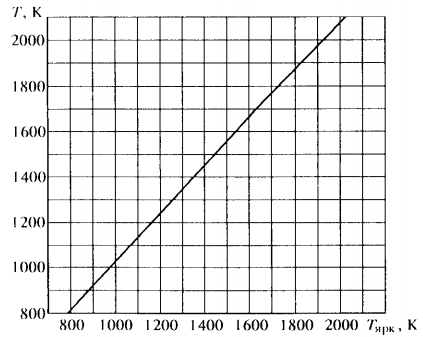
\includegraphics[width=10cm]{fig2.PNG}
    \caption{График зависимости $T = f(T_{br})$ для вольфрам}
    \label{fig:vac}
\end{figure}


Также в данной работе измеряется температура вольфрамовой нити в лампе накала. Запишем закон излучения АЧТ:
\begin{equation}
    W = \sigma S (T^4 - T_0^4),
\end{equation}
где $W$ - потребляемая нитью электрическая мощность, $S$ - площадь излучающей поверхности нити, $T$ - температура нити, $T_0$ - температура окружающей среды. Однако, вольфрамовая нить в лампе накаливания не является АЧТ, из-за чего вводится $\varepsilon_T$ - коэффициент серости тела. В таком случае, с учётом $T^4 >> T_0 ^ 4$:
\begin{equation}
    W = \varepsilon_T S \sigma T^4
\end{equation}
Проверим выполнение закона Стефана-Больцмана в данной работе, а также определим постоянную Стефана-Больцмана.


\section * {Оборудование и инструментальные погрешности}

Исследуемые в работе образцы:
\begin{itemize}
    \item \textbf{модель абсолютно чёрного тела} - керамическая трубка, закрытая с одного конца и окружённая для теплоизоляции внешним кожухом. Температура в трубке измеряется с помощью термопары хромель-алюмель
    \item \textbf{вольфрамовая нить электрической лампы накаливания}
    \item \textbf{трубка с кольцами из материалов с различной излучательной способностью}
    \item \textbf{неоновая лампочка}
\end{itemize}

\begin{figure}[h]
    \centering
    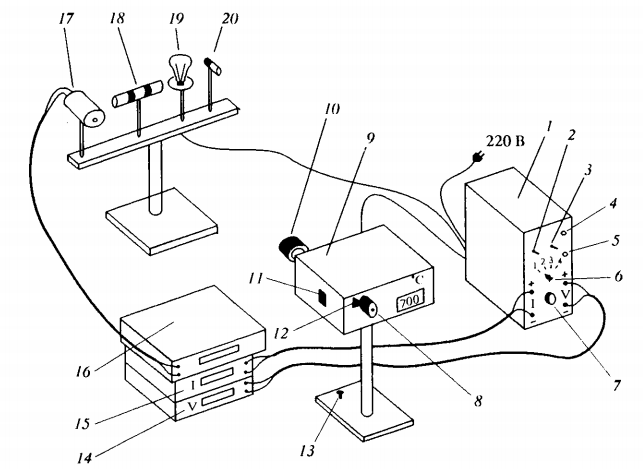
\includegraphics[width=0.8\linewidth]{fig1.PNG}
    \caption{Схема установки}
    \label{fig:scheme}
\end{figure}

\newpage

\section * {Результаты измерений и обработка данных}

\subsection * {Изучение оптического пирометра}

Нагреем модель АЧТ, включим пирометр и прогреем его нить. Измерим температуру модели АЧТ оптическим пирометром и термопарой и занесём данные в таблицу, учитывая, что термопара измеряет температуру АЧТ относительно комнатной температуры:

\begin{table}[h!]
\caption{Температура АЧТ, измеренная разными способами}
\begin{tabular}{lllll}
\hline
\multicolumn{1}{|l|}{$T_\text{п}, ^\circ C$} & \multicolumn{1}{l|}{1060}  & \multicolumn{1}{l|}{1071}  & \multicolumn{1}{l|}{1071}  & \multicolumn{1}{l|}{1077}  \\ \hline
\multicolumn{1}{|l|}{$\varepsilon_\text{т}, \text{мВ}$}    & \multicolumn{1}{l|}{40.10} & \multicolumn{1}{l|}{40.20} & \multicolumn{1}{l|}{40.42} & \multicolumn{1}{l|}{40.37} \\ \hline
\multicolumn{1}{|l|}{$T_\text{т}, ^\circ C$}    & \multicolumn{1}{l|}{1007}  & \multicolumn{1}{l|}{1015}  & \multicolumn{1}{l|}{1030}  & \multicolumn{1}{l|}{1028}  \\ \hline
                           &                            &                            &                            &                           
\end{tabular}
\end{table}

Такое большое расхождение в результатах можно объяснить тем, что оба способа измерения температуры имеют большую погрешность, но в целом результаты можно считать удовлетворительными.

Из данного пункта можно заметить, термодинамическая температура при переводе из яркостной по \ref{fig:vac} отличается от измеренной термопарой ещё больше, чем яркостная. Поэтому не буду использовать данный график в дальнешей работе.

\subsection * {Измерение температуры накалённых тел}

Нагреем керамическую трубку с кольцами на ней и измерим их яркостную температуру. Получили:

\[ T_{\text{трубки}} = 1012 ^\circ C\]
\[ T_{\text{правого кольца}} = 884 ^\circ C\]
\[ T_{\text{левого кольца}} = 884 ^\circ C\]

Разницу в температурах трубки и колец можно объяснить различием коэффициента серости $\varepsilon$ материалов. Кольца же показали одинаковую температуру, хотя в описании утверждается, что материалы разные. На некоторых других установках было 4 кольца, так что этот пункт лабораторной работы можно считать спорным. Также, возможно, фактическая температура колец была разная, но разница их цвета была неразличима для глаза экспериментатора.

\subsection * {Измерение температуры накалённых тел}

\subsubsection * {Проверка закона Стефана-Больцмана}

Постепенно увеличивая напряжение на лампе накаливаниия, снимем значения яркостной температуры, измеренной пирометром, а так же силу тока и напряжение на лампе накаливания. Работаем в диапазоне $920-2100 ^\circ C$. \par

Представим зависимость $W = \varepsilon_T S \sigma T^4$ в логарифмическом масштабе

\[ ln(W) = ln(\varepsilon_T S \sigma) + n \times ln(T) \]

и построим график этой зависимости.

\begin{figure}
    \centering
    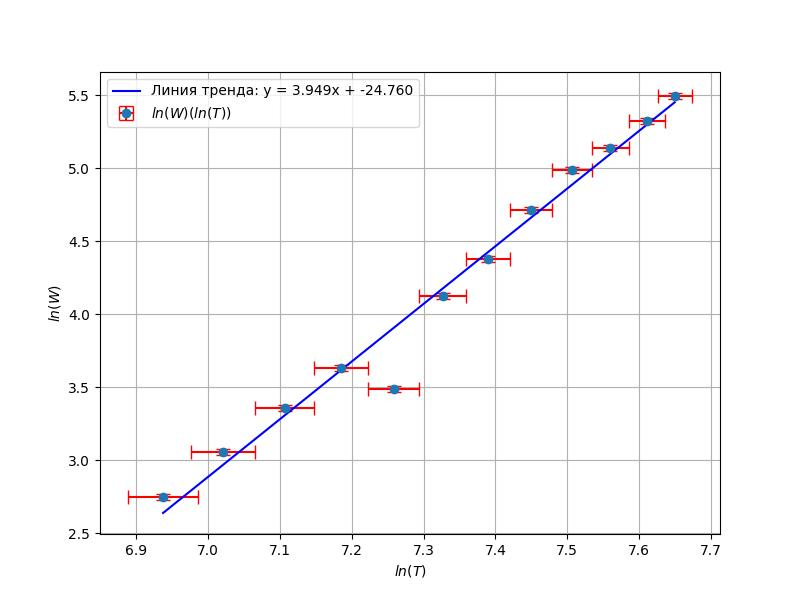
\includegraphics[width=1\linewidth]{plot.jpg}
    \caption{График зависимости W(T) в логарифмическом масштабе}
    \label{fig:plt}
\end{figure}

Как видим из графика, $n = 3.949 \pm 0.03$, что очень близко к теоретическому значению $n = 4$. Так что, можно заключить, что закон Стефана-Больцмана выполняется.

\subsubsection * {Вычисление постоянной Стефана-Больцмана и постоянной Планка}

Определим постоянную Стефана-Больцмана, используя значения термодинамической температуры выше 1700$^{\circ}$C и соответствующую мощность ($S = 5.0$ см$^2$). После усреднения получим:

\[\sigma = \frac{W}{\varepsilon_T S T^4} = (7.05 \pm 1.21) \cdot 10^{-12} \frac{Вт}{см^2 \cdot K^4}\]

Определённое значение постоянной Стефана-Больцмана близко к теоретическому:

\[\sigma_{th} = 5.67\cdot 10^{-12} \frac{Вт}{см^2 \cdot K^4}\]

Теперь оценим значение постоянной Планка:

\[ h = \sqrt[3]{\frac{2 \pi^5 k_B^4}{15 c^2 \sigma}} = (6.14 \pm 1.05) \cdot 10^{-34} \text{Дж} \cdot \text{с}\]

что в пределах погрешности совпадает с теоретическим значением.

Измеренные данные для наглядности представим в таблице \ref{tab:data}. Температура представлена в $^\circ C$, но расчёты проводились в K.

\begin{table}[h!]
\caption{Таблица с данными}
\label{tab:data}
\begin{tabular}{|l|l|l|l|l|}
\hline
T, $^\circ C$    & U, В      & I, А     & $\sigma \cdot 10^{-12}, \frac{Вт}{см^2 \cdot K^4}$  & $\Delta \sigma \cdot 10^{-12}, \frac{Вт}{см^2 \cdot K^4}$ \\ \hline
920  & 16.65  & 0.625 & -    & -    \\ \hline
1030 & 22.21  & 0.700 & -    & -    \\ \hline
1120 & 27.62  & 0.768 & -    & -    \\ \hline
1220 & 33.99  & 0.845 & -    & -    \\ \hline
1320 & 40.84  & 0.922 & -    & -    \\ \hline
1420 & 31.48  & 1.036 & -    & -    \\ \hline
1520 & 56.47  & 1.093 & -    & -    \\ \hline
1620 & 66.79  & 1.192 & -    & -    \\ \hline
1720 & 83.13  & 1.343 & 6.77 & 1.24 \\ \hline
1820 & 99.01  & 1.477 & 7.29 & 1.27 \\ \hline
1920 & 109.45 & 1.555 & 7.04 & 1.17 \\ \hline
2020 & 123.23 & 1.664 & 7.10 & 1.13 \\ \hline
2100 & 137.67 & 1.767 & -    & -    \\ \hline
\end{tabular}
\end{table}

\newpage

\subsection * {Измерение "яркостной температуры" неоновой лампочки}

С помощью пирометра измерим "яркостную температуру" неоновой лампочки и получим результат $T_H = 1009 ^\circ C$. Дотронувшись до лампочки и оставшись без ожога осознаем, что термодинамическая температура значительно ниже. Это явление можно объяснить тем, что пирометр расчитан на измерение температуры АЧТ и его принцип работы основан на принципах излучения АЧТ. Неоновая лампочка очень далека от модели АЧТ и её излучение имеет совершенно другую, не термодинамическую природу, поэтому и получается такой результат. 

\section * {Вывод}

При помощи модели абсолютно черного тела (АЧТ) провели измерения температуры оптическим пирометром и термопарой, исследовали излучение накаленных тел с различной испускательной способностью, определили постоянные Планка и Стефана–Больцмана. \par

В целом, качественные результаты полностью совпадают с теорией. Количественные же можно назвать удовлетворительными, но стоит отметить высокую погрешность. Её можно объяснить множеством пренебрежений в рабооте по сравнению с теорией, невысокой точностью измерительных приборов а так же большим влиянием человеческого фактора.


\begin{thebibliography}{9}
	\bibitem{Siv} Сивухин Д. В. \emph{Общий курс физики. Том 5 Атомная и ядерная физика}, 2004
	\bibitem{kir} Кириченко Н. А. \emph{Начальные главы квантовой механики}, 2014
	\bibitem{max} \emph{Лабораторный практикум по общей физике. Квантовая физика.} под ред. Ю. М. Ципенюка
\end{thebibliography}
\end{document}

















